\documentclass[border=6pt]{standalone}
\usepackage{lmodern}
\usepackage[T1]{fontenc}
\usepackage{amsmath}
\usepackage{bm}
\usepackage{xcolor}
\usepackage{tikz}
\usetikzlibrary{arrows.meta,positioning,decorations.pathreplacing}
\definecolor{cgray}{HTML}{6E6C66}
\definecolor{cblue}{HTML}{2F7DC8}
\definecolor{camber}{HTML}{E0891E}
\definecolor{cgreen}{HTML}{4E8E2A}
\definecolor{cred}{HTML}{B23B3B}
\definecolor{cink}{HTML}{2B2B2B}
\tikzset{
  >={Stealth[length=2.6mm]},
  arm/.style={rounded corners=2pt,draw,line width=0.8pt,align=center,
              minimum width=3.3cm,minimum height=0.95cm,inner sep=2pt},
  outer/.style={rounded corners=5pt,draw=cink!45,line width=0.9pt},
  ttl/.style={font=\bfseries\small,text=cink},
  lbl/.style={font=\footnotesize,text=cink!75},
  flow/.style={->,line width=1.2pt},
}
\begin{document}
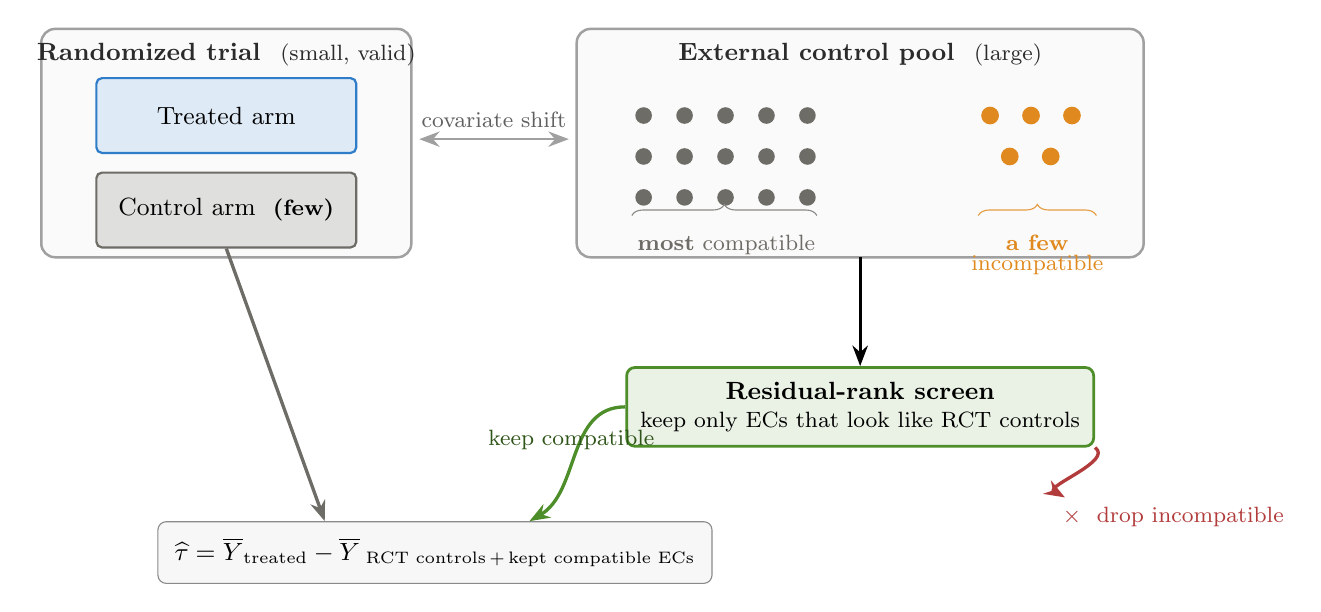
\begin{tikzpicture}[font=\small]

% ================= TOP-LEFT: randomized trial =================
\draw[outer,fill=black!2] (-0.3,4.45) rectangle (4.4,7.35);
\node[ttl] at (2.05,7.02) {Randomized trial \ \mdseries\footnotesize(small, valid)};
\node[arm,fill=cblue!16,draw=cblue] (trt) at (2.05,6.25) {Treated arm};
\node[arm,fill=cgray!22,draw=cgray] (ctr) at (2.05,5.05) {Control arm \ \footnotesize\textbf{(few)}};

% ================= TOP-RIGHT: external pool =================
\draw[outer,fill=black!2] (6.5,4.45) rectangle (13.7,7.35);
\node[ttl] at (10.1,7.02) {External control pool \ \mdseries\footnotesize(large)};
% compatible majority (gray block)
\foreach \r in {0,1,2}\foreach \c in {0,1,2,3,4}
   \fill[cgray] (7.35+\c*0.52,6.25-\r*0.52) circle (3.0pt);
% incompatible minority (few amber)
\foreach \c in {0,1,2}\fill[camber] (11.75+\c*0.52,6.25) circle (3.2pt);
\foreach \c in {0,1}\fill[camber] (12.0+\c*0.52,5.73) circle (3.2pt);
\draw[decorate,decoration={brace,amplitude=4pt},cgray!80] (7.2,4.98) -- (9.55,4.98);
\node[lbl,text=cgray,below] at (8.4,4.86) {\textbf{most} compatible};
\draw[decorate,decoration={brace,amplitude=4pt},camber!85] (11.6,4.98) -- (13.1,4.98);
\node[lbl,text=camber,below,align=center] at (12.35,4.86) {\textbf{a few}\\[-2pt]incompatible};

% covariate shift (single light annotation)
\draw[<->,cink!45,line width=0.8pt] (4.5,5.95) -- (6.4,5.95);
\node[lbl,above] at (5.45,5.98) {covariate shift};

% ================= SCREEN =================
\node[rounded corners=3pt,draw=cgreen,fill=cgreen!12,line width=1.0pt,
      align=center,minimum height=1.0cm,inner sep=5pt] (scr) at (10.1,2.55)
      {\textbf{Residual-rank screen}\\[-1pt]\footnotesize keep only ECs that look like RCT controls};
\draw[flow] (10.1,4.45) -- (scr.north);
\draw[flow,cred] (scr.south east) to[out=-35,in=150] (12.7,1.4);
\node[cred,font=\footnotesize,anchor=west] at (12.55,1.15) {$\times$\ \ drop incompatible};

% ================= ESTIMAND (bottom) =================
\node[rounded corners=3pt,draw=cink!55,fill=black!3,align=center,inner sep=6pt] (est) at (4.7,0.7)
   {$\displaystyle \widehat\tau=\overline{Y}_{\text{treated}}-\overline{Y}_{\;\text{RCT controls}\,+\,\text{kept compatible ECs}}$};
\draw[flow,cgray] (ctr.south) -- ([xshift=-1.4cm]est.north);
\draw[flow,cgreen] (scr.west) to[out=180,in=30] node[lbl,text=cgreen!60!black,above,pos=0.55]{keep compatible} ([xshift=1.2cm]est.north);

\end{tikzpicture}
\end{document}
